\chapter{Proof of the Upper and Lower Bounds}
\myTop{The upper and lower bound of the \rubik{} will be presented and explained in this chapter. The bounds needs to be proven, in order for it to be recognized.}

\begin{comment}
The lower bound is the number of twists required to solve the \rubik{} in the position which requires the most twists to solve.
The upper bound is the lowest number of twists proven to solve a \rubik{} in any position.
Both bounds can be seen on figure \ref{fig:upperLowerBound}.
As the figure shows, the upper bound closes in on the lower bound.
The graph show that the two lines will converge at some point.

Proofs of the upper bound have been published several times, and it has been lowered each time.
A major breakthrough was when Thistlethwaite's algorithm was proven to be able to solve an arbitrary \rubik{} in 52 twists or less \cite{jaapthistle}.
Since then a lot of progress has been made in the field.
This section describes this progression.

\begin{figure}[ht]
	\centering
		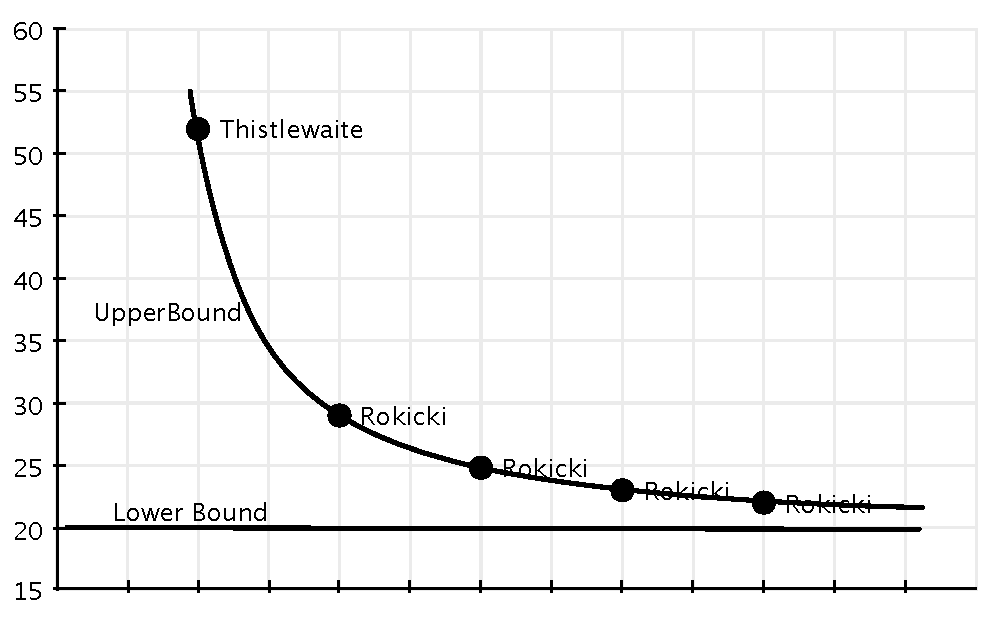
\includegraphics[scale = 0.7]{input/pics/bounds.pdf}
	\caption{\myCaption{The current upper and lower bound. The x-axis depicts time and y-axis moves.}}
	\label{fig:upperLowerBound}
\end{figure}
\end{comment}

%\section{Set Solver}
\label{sec:setSolver}
The algorithm used to prove the current lowest upper bound is known as a set solver and uses Kociemba's algorithm. The set solver is a viable method for proving the upper bound because it does not solve every single cube but a whole set of cubes at the time as the name suggests. This means that it solves approximately 19.5 billion cubes at a time.
The set solver does this by finding all the move sequences of a relabeled cube of the distance $d$ that transforms the cube into \m{H}. 
The algorithm set solver is described in pseudo code below in algorithm \ref{alg:setSolver}.%All the move sequences to transform the unlabeled cube to $e$ is in a database so it is fast to find the shortest move sequence, once the move sequence to \m{H} has been found.

\begin{algorithm}[!h]                     
\caption{Set Solver \cite{rokicki09}}          
\label{alg:setSolver}        
\begin{algorithmic}[1]
\STATE {$f=\oslash$}
\STATE {$d=0$}
\WHILE {true} 
		\IF {$d \leq m$}
			\FOR {$b \in S^d$}
				\IF {$r(ab) = r(e)$}
					\STATE {$f = f \cup ab$}
				\ENDIF
			\ENDFOR
		\ENDIF
		\IF {$f = H$}
			\STATE {return $d$}
		\ENDIF
	\STATE {$d = d + 1$}
	\STATE {$f = f \cup fA$}
	\IF {$f = H$}
		\STATE {return $d$}
	\ENDIF
\ENDWHILE
\end{algorithmic}
\end{algorithm}

First in the set solver two variables are initialized. The first one \m{f} is a set that can hold all the positions of \m{H} is set to an empty set. The second variable is the distance $d$, which is the distance from a scrambled position $a$ to a position in \m{H}. This distance $d$ is initially set to $0$.

Next the \textbf{while} loop is run. It will run until $d$ is returned, which is when all positions in \m{H} has been found.

$m$ is the maximum number of \m{S} moves performed from the position $a$. When $d$ is equal to $m$ only \m{A} moves are performed.
If $d$ is lower than or equal to $m$ a for loop will be run. This loop performs all possible move sequences of the the length $d$, and adds the position $ab$ to \m{f} if it is a position in \m{H}. 
For the sake of efficiency move sequences that give the exact same position more than once are not used. If a move sequence contained F F', that part would  of the move sequence would be unnecessary. 

If \m{f} is equal to \m{H} all positions in \m{H} have been found, $d$ is returned and the algorithm has finished. 
If this is not the case, $d$ is incremented by one. 
The different \m{A} moves are performed on all the current \m{H} positions in \m{f} and the new \m{H} positions are saved in \m{f}.
If \m{f} contains all positions in \m{H}, $d$ is returned -- if not the while loop continues.



When the algorithm has finished all the different possible \m{H} positions should be saved, if the maximum distance $m$ is set sufficiently high. The theoretically highest number of twists needed to transform any scrambled cube into \m{H} is 12, but more positions are found in the for loop if $m$ is set higher. This is because the set solver both performs \m{A} moves on a cube in \m{H}, which gives more \m{H} positions. The set solver also performs moves that transforms a cube in \m{H} to a cube not in \m{H} and then back again by using \m{S} moves.

\myTail{The current upper bound is proven to be 22 twists by Thomas Rokicki using a modified version of Kociemba's optimal solver, solving a set at a time rather than just a single \rubik{}. The upper bound may be lowered in the future, it is however currently difficult due to how much CPU time is needed. The current lower bound has been proven to be 20 twists}